\chapter{التحليل الطيفي لتعيين البنية}\label{ch:b1:structure-spectroscopy}

يسلّم صانع عطور المختبر سائلًا عديم اللون تفوح منه رائحة
الأناناس ويسأل عن ماهيته. قبل خمسين عامًا كان الجواب يتطلب
أسابيع من تفاعلات التفكيك. أما اليوم فيكفيه عشر دقائق: يعطي
التحليل العنصري الصيغة، ويسمّي طيف الأشعة تحت الحمراء
المجموعة الوظيفية، ويبيّن طيف الرنين المغناطيسي النووي للبروتون
كيف ترتبط الذرات. يشرح هذا الفصل كيف يُقرأ كل طيف
--- ما يفعله ضوء كل منطقة بالجزيء، وأي سمات الطيف
تحمل أي جزء من البنية --- وينتهي بجزيء
الأناناس ذاك.

\begin{recall}
قاس المجلد المدرسي (الصفان الحادي عشر والثاني عشر) الامتصاصيات بمقياس
الطيف الضوئي واستعمل قانون بير--لامبرت لإيجاد التراكيز،
وتعرّف المجموعات الوظيفية من جداول حزم الأشعة تحت الحمراء، وقرأ
أطياف رنين مغناطيسي نووي بروتونية بسيطة (عدد الإشارات، \omterm{def:b1:structure-spectroscopy:integration}{والتكامل}، وقاعدة $n + 1$). أما الروابط الأحادية والثنائية والثلاثية والرابطة $\pi$ فهي روابط
\cref{ch:b1:lewis-resonance-vsepr}.
\end{recall}

\section{التحليل الطيفي في المجالين فوق البنفسجي والمرئي: الترافق واللون}

\begin{definition}[الامتصاصية وقانون بير--لامبرت]\label{def:b1:structure-spectroscopy:absorbance}
من أجل ضوء شدته $I_0$ يدخل محلولًا وشدته $I$ عند خروجه منه، تكون
\emph{الامتصاصية}\index{امتصاصية} $A = \log(I_0/I)$. ومن أجل محلول
مخفف لنوع ماص واحد، $A = \varepsilon\,\ell\,c$ (قانون
بير--لامبرت)، حيث $\ell$ طول المسار، و$c$
التركيز و$\varepsilon$ \emph{معامل الامتصاص
المولي}\index{معامل الامتصاص المولي}، وهو خاصية
للنوع عند ذلك الطول الموجي.
\end{definition}

يمتص الجزيء الضوء فوق البنفسجي أو المرئي حين تساوي طاقة الفوتون
الفجوة بين أعلى مستويات إلكترونية مشغولة وأدنى مستويات فارغة
لروابطه. ففي الروابط $\sigma$ تكون الفجوة كبيرة ويقع
الامتصاص بعيدًا في فوق البنفسجي؛ وتمتص الروابط $\pi$ أقرب إلى
المرئي، وتمتص سلسلة من روابط ثنائية وأحادية متناوبة عند
أطوال موجية أكبر كلما طالت السلسلة.

\begin{definition}[النظام المترافق، حامل اللون، قمة الامتصاص]\label{def:b1:structure-spectroscopy:conjugation}
\emph{النظام المترافق}\index{نظام مترافق} سلسلة من الذرات
يحمل كل منها مدارًا $p$ في نظام $\pi$، كما في الروابط الثنائية
والأحادية المتناوبة (البوتا-1,3-ثنائي الإين، البنزين). ومجموعة الذرات
المسؤولة عن امتصاص ما هي \emph{حامل اللون}\index{حامل اللون}؛
والطول الموجي الذي تكون عنده امتصاصيتها أكبر ما يمكن هو
\emph{قمة الامتصاص}\index{قمة الامتصاص}، $\lambda_{\max}$.
\end{definition}

تمتد مستويات \omterm{def:b1:structure-spectroscopy:conjugation}{النظام المترافق} على السلسلة كلها وتتقارب
كلما طالت السلسلة، كما تتقارب مستويات جسيم في
صندوق أطول: فتزداد $\lambda_{\max}$ مع الترافق. ولا يمتص الإيثين
والبوتاديين إلا في فوق البنفسجي؛ أما الروابط الثنائية المترافقة الإحدى عشرة
في الكاروتين-$\beta$ فتنقل الامتصاص إلى الجزء الأزرق من
المرئي. وتبدو المادة باللون المتتام للضوء الذي
تمتصه: فالكاروتين الذي يمتص الأزرق والبنفسجي يبدو برتقاليًا.

\begin{omfigure}
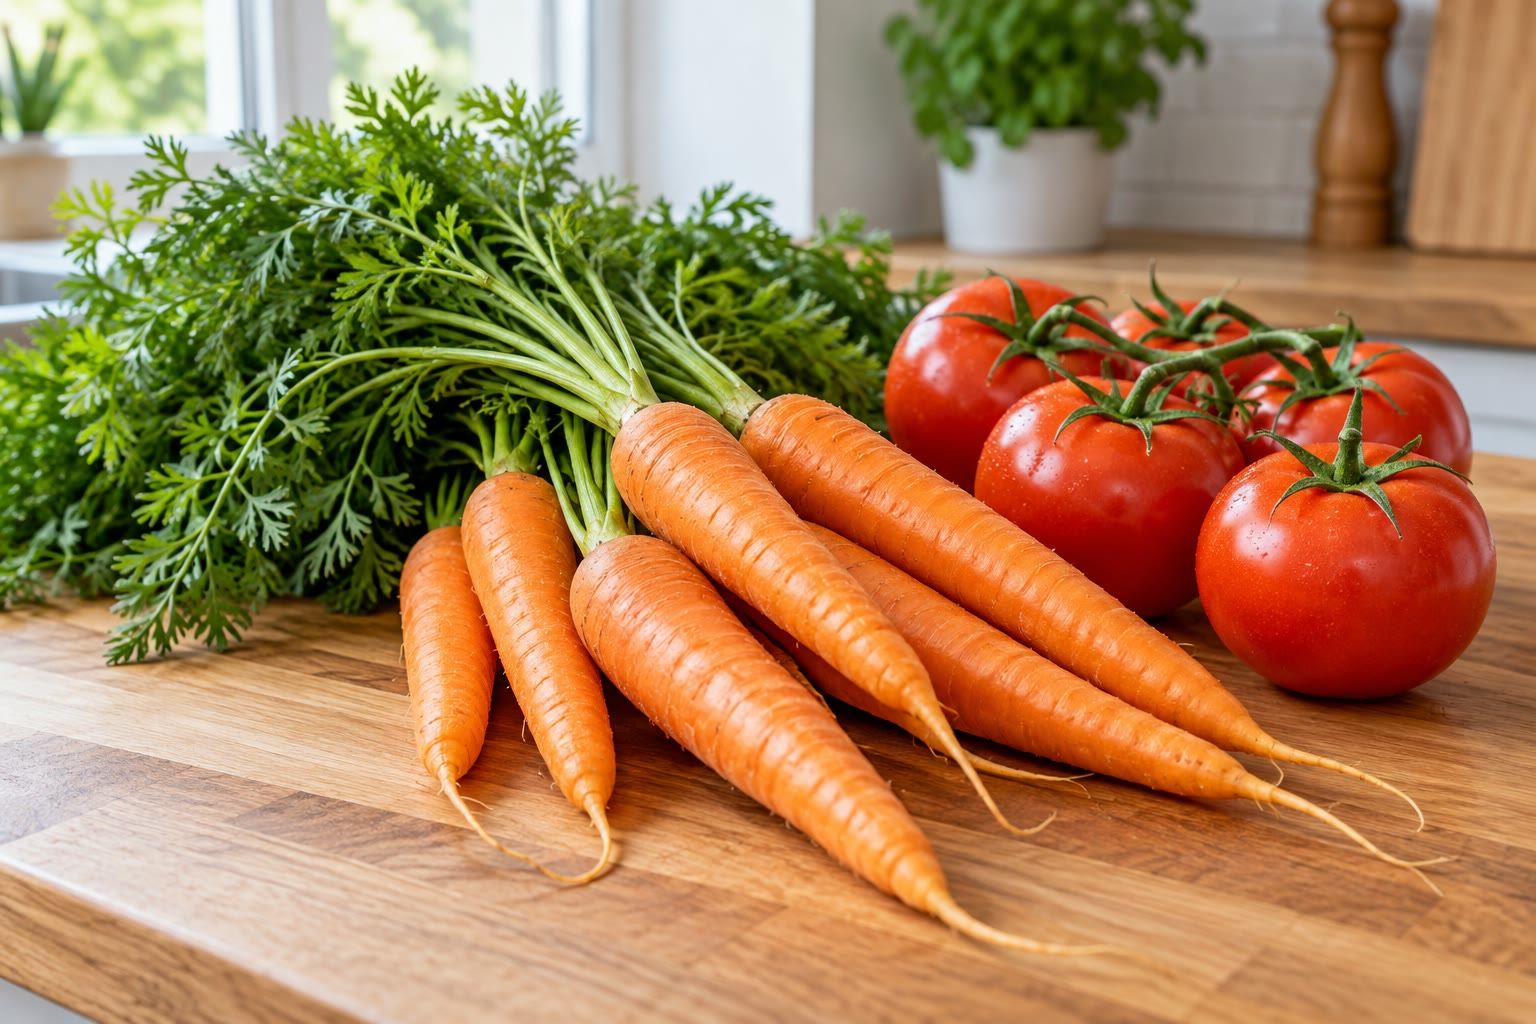
\includegraphics[width=0.55\linewidth]{images/book2/ai/b1-17-carrots-tomatoes.jpg}

{\small يدين الجزر والطماطم بلونيهما لجزيئات مترافقة طويلة،
هي الكاروتينات والليكوبين، تمتص الضوء الأزرق والأخضر وتمرر
البرتقالي والأحمر.}
\end{omfigure}

\begin{omfigure}
\begin{tikzpicture}[font=\small]
  \foreach \a/\c/\n in {90/red/{أحمر}, 30/orange/{برتقالي}, -30/yellow/{أصفر}, -90/green!70!black/{أخضر}, -150/blue/{أزرق}, 150/violet/{بنفسجي}} {
    \fill[\c] (0,0) -- (\a-30:1.4) arc[start angle=\a-30, end angle=\a+30, radius=1.4] -- cycle;
    \node at (\a:1.85) {\n};
  }
  \draw[<->, thick] (-150:0.9) -- (30:0.9);
  \node[align=left, anchor=west] at (2.6,0.3) {\babelsublr{\foreignlanguage{arabic}{يمتص الأزرق} $\Rightarrow$ \foreignlanguage{arabic}{يبدو برتقاليًا}}\\\foreignlanguage{arabic}{الألوان المتتامة متقابلة}\\\foreignlanguage{arabic}{على الدائرة}};
\end{tikzpicture}

{\small دائرة الألوان. اللون المرئي هو متمم اللون
الممتص: فالمحلول الذي يمتص في الأزرق يبدو برتقاليًا.}
\end{omfigure}

\section{التحليل الطيفي بالأشعة تحت الحمراء بتعمق}

\begin{definition}[العدد الموجي، النفاذية، منطقة البصمة]\label{def:b1:structure-spectroscopy:wavenumber}
تُرسم أطياف الأشعة تحت الحمراء بدلالة \emph{العدد الموجي}\index{عدد موجي}
$\tilde\nu = 1/\lambda$، بالوحدة \unit{cm^{-1}}، المتناسب مع طاقة
الفوتون. والإحداثي الرأسي هو \emph{النفاذية}\index{نفاذية}
$T = I/I_0$، بالنسبة المئوية، فتتجه الحزم نحو الأسفل. وتحت نحو
\qty{1500}{cm^{-1}} تكوّن حزم كثيرة متراكبة، مميزة للجزيء
كله لا لرابطة واحدة، \emph{منطقة
البصمة}\index{منطقة البصمة}.
\end{definition}

تمتص الرابطة ضوء الأشعة تحت الحمراء عند التردد الذي تهتز به.
وكما في كتلتين يصل بينهما نابض، كلما كانت الرابطة أصلب
والذرتان أخف، كان \omterm{def:b1:structure-spectroscopy:wavenumber}{العدد الموجي} أعلى: الروابط مع الهيدروجين (O--H، C--H)
فوق \qty{2800}{cm^{-1}}، والروابط الثلاثية قرب 2200، والروابط الثنائية قرب
1700--1600، والروابط الأحادية بين ذرات أثقل تحت 1300. ويعطي الجدول
مواضع مقيسة لجزيئات هذا الفصل، في \omterm{def:b1:extent-q-and-k:system}{الطور} الغازي،
حيث تكون الجزيئات منعزلة.

\begin{omfigure}
\begin{tabular}{llr}
\hline
الجزيء & الرابطة & $\tilde\nu$ (\unit{cm^{-1}}) \\
\hline
الإيثانول & O--H & 3666 \\
الإيثانول & C--H & 2978 \\
الإيثانول & C--O & 1060 \\
البروبانون & C=O & 1738 \\
حمض الإيثانويك & O--H & 3582 \\
حمض الإيثانويك & C=O & 1788 \\
إيثانوات الإيثيل & C=O & 1764 \\
إيثانوات الإيثيل & C--O & 1238 \\
\hline
\end{tabular}

\smallskip
{\small قمم الحزم في أطياف الأشعة تحت الحمراء \omterm{def:b1:extent-q-and-k:system}{للطور} الغازي. في السوائل، توسّع \omterm{def:b1:intermolecular-forces-solvents:hbond}{الروابط
الهيدروجينية} حزم O--H وتنقلها إلى أعداد موجية أدنى،
وتنزاح حزم C=O للأحماض نحو الأدنى حين تتزاوج جزيئات الحمض.}
% ledger: ir:ethanol-OH, ir:ethanol-CH, ir:ethanol-CO, ir:propanone-CO, ir:ethanoic-OH, ir:ethanoic-CO, ir:ethylethanoate-CO, ir:ethylethanoate-COC
\end{omfigure}

\begin{omfigure}
\begin{tikzpicture}
\begin{axis}[name=i1, width=0.86\linewidth, height=3.2cm, xmin=500, xmax=4000, x dir=reverse, ymin=0, ymax=105, ytick={0,50,100}, ylabel={\babelsublr{$T$ (\%)}}, tick label style={font=\scriptsize}, label style={font=\small}, xticklabels={}]
\addplot[omDef, thick] table[x=nu, y=T] {figdata/out/bachelor-1-spectra-ir-ethanol.dat};
\node[font=\scriptsize, anchor=west] at (axis cs:2600,25) {الإيثانول};
\end{axis}
\begin{axis}[name=i2, at={(i1.south)}, anchor=north, yshift=-0.25cm, width=0.86\linewidth, height=3.2cm, xmin=500, xmax=4000, x dir=reverse, ymin=0, ymax=105, ytick={0,50,100}, ylabel={\babelsublr{$T$ (\%)}}, tick label style={font=\scriptsize}, label style={font=\small}, xticklabels={}]
\addplot[omProp, thick] table[x=nu, y=T] {figdata/out/bachelor-1-spectra-ir-propanone.dat};
\node[font=\scriptsize, anchor=west] at (axis cs:2600,25) {البروبانون};
\end{axis}
\begin{axis}[at={(i2.south)}, anchor=north, yshift=-0.25cm, width=0.86\linewidth, height=3.2cm, xmin=500, xmax=4000, x dir=reverse, ymin=0, ymax=105, ytick={0,50,100}, ylabel={\babelsublr{$T$ (\%)}}, tick label style={font=\scriptsize}, label style={font=\small}, xlabel={\foreignlanguage{arabic}{العدد الموجي بالوحدة \unit{cm^{-1}}}}]
\addplot[omMeth, thick] table[x=nu, y=T] {figdata/out/bachelor-1-spectra-ir-ethanoic.dat};
\node[font=\scriptsize, anchor=west] at (axis cs:2600,25) {حمض الإيثانويك};
\end{axis}
\end{tikzpicture}

{\small أطياف الأشعة تحت الحمراء للإيثانول والبروبانون وحمض الإيثانويك،
محاكاة انطلاقًا من مواضع الحزم المقيسة في الجدول (ارتفاعات الحزم
وعروضها تخطيطية). حزمة C=O قرب \qty{1750}{cm^{-1}} وحزمة O--H
فوق \qty{3500}{cm^{-1}} تميّزان المجموعات الوظيفية الثلاث من
النظرة الأولى.}
\end{omfigure}

\section{الرنين المغناطيسي النووي للبروتون: الانزياح الكيميائي والتكامل}

في مجال مغناطيسي قوي يكون للبروتون مستويا طاقة؛ والموجات الراديوية
ذات التردد المناسب تجعله ينقلب من أحدهما إلى الآخر. وهذا التردد
متناسب مع المجال المغناطيسي الذي يحسّه البروتون فعلًا، والذي
تخفّضه الإلكترونات المحيطة به قليلًا. فالبروتونات في بيئات كيميائية
مختلفة ترنّ إذن عند ترددات مختلفة قليلًا.

\begin{definition}[الانزياح الكيميائي، الحجب، البروتونات المتكافئة]\label{def:b1:structure-spectroscopy:chemical-shift}
\emph{الانزياح الكيميائي}\index{انزياح كيميائي} لبروتون هو
$\delta = (\nu - \nu_{\text{مرجع}})/\nu_0 \times 10^6$، بالوحدة \unit{ppm}، حيث
$\nu$ تردد رنينه، و$\nu_{\text{مرجع}}$ تردد رنين بروتونات
رباعي ميثيل السيليكون و$\nu_0$ تردد تشغيل
المطياف. وتخفيض المجال عند نواة بفعل إلكتروناتها هو
\emph{حجبها}\index{حجب (رنين مغناطيسي نووي)}: فالمجموعات المجاورة الساحبة للإلكترونات
(O، والهالوجينات، وC=O) تزيل الحجب عن البروتون وترفع $\delta$ له.
و\emph{البروتونات المتكافئة}\index{بروتونات متكافئة} بروتونات يبادل بينها
تناظر في الجزيء أو دوران سريع؛ ولها
الانزياح نفسه.
\end{definition}

\begin{proposition}[الانزياح لا يتعلق بالمطياف]\label{prop:b1:structure-spectroscopy:shift-field-independent}
\omterm{def:b1:structure-spectroscopy:chemical-shift}{الانزياح الكيميائي} لبروتون هو نفسه على مطيافات ذات
مجالات مختلفة.
\end{proposition}

\begin{proof}
كل من $\nu$ و$\nu_{\text{مرجع}}$ متناسب مع المجال المطبَّق
$B_0$ (كل منهما مضروب في معامل الحجب الخاص به)، وكذلك $\nu_0$.
فالنسبة $(\nu - \nu_{\text{مرجع}})/\nu_0$ إذن مستقلة عن
$B_0$. أما الفروق بالهرتز فتكبر، على العكس، مع المجال.
\end{proof}

\begin{definition}[التكامل]\label{def:b1:structure-spectroscopy:integration}
\emph{تكامل}\index{تكامل} الإشارة هو مساحتها، وتُقرأ
على الطيف ارتفاعًا لمنحنى درجي؛ والمساحات متناسبة مع
أعداد البروتونات التي تعطي الإشارات.
\end{definition}

\section{الاقتران سبين--سبين}

\begin{definition}[الاقتران سبين--سبين، ثابت الاقتران، متعدد الخطوط]\label{def:b1:structure-spectroscopy:coupling}
عبر الروابط، تغيّر الحالة المغناطيسية لبروتون تغييرًا طفيفًا
المجال الذي تحسّه البروتونات على الكربونات المجاورة: وهذا
\emph{الاقتران سبين--سبين}\index{اقتران سبين--سبين} يشطر كل إشارة
إلى \emph{متعدد خطوط}\index{متعدد خطوط} تفصل بين خطوطه مسافة
\emph{ثابت الاقتران}\index{ثابت الاقتران} $J$، بالهرتز. والبروتونان
المقترنان أحدهما بالآخر يُظهران قيمة $J$ نفسها؛ \omterm{def:b1:structure-spectroscopy:chemical-shift}{والبروتونات المتكافئة}
لا يشطر بعضها إشارة بعض.
\end{definition}

\begin{proposition}[قاعدة \texorpdfstring{$n + 1$}{n + 1}]\label{prop:b1:structure-spectroscopy:n-plus-one}
البروتون (أو مجموعة \omterm{def:b1:structure-spectroscopy:chemical-shift}{البروتونات المتكافئة}) المقترن بقيمة $J$ نفسها مع
$n$ جارًا متكافئًا يعطي $n + 1$ خطًا، تفصل بينها $J$،
وشدّاتها النسبية هي المعاملات الثنائية $\binom{n}{k}$، من $k = 0$ إلى
$n$ (\emph{قاعدة $n + 1$}\index{قاعدة $n + 1$}).
\end{proposition}

\begin{proof}
كل جار في واحدة من حالتي سبين، تزيح الخط المرصود بمقدار
$+J/2$ أو $-J/2$. ومع $n$ جارًا يكون الانزياح $(k - n/2)J$، حيث $k$
عدد الجيران في الحالة الأولى: $n + 1$ قيمة، متساوية التباعد بمقدار $J$.
ولأن الحالتين متساويتا الإشغال تقريبًا، فإن التركيبات $2^n$ كلها
متساوية الاحتمال، ويمكن أن يكون $k$ منها في الحالة الأولى بعدد
$\binom{n}{k}$ من الطرائق.
\end{proof}

\begin{omfigure}
\begin{tikzpicture}[font=\small, x=0.85cm, y=0.5cm]
  % quartet: three neighbours, each split +-J/2 (J = 1.5 units)
  \draw[thick] (0,4) -- (0,3.4);
  \foreach \x in {-0.75,0.75} \draw (0,3.4) -- (\x,2.4);
  \foreach \a/\b in {-0.75/-1.5, -0.75/0, 0.75/0, 0.75/1.5} \draw (\a,2.4) -- (\b,1.4);
  \foreach \a/\b in {-1.5/-2.25, -1.5/-0.75, 0/-0.75, 0/0.75, 1.5/0.75, 1.5/2.25} \draw (\a,1.4) -- (\b,0.4);
  \foreach \x/\h in {-2.25/1, -0.75/3, 0.75/3, 2.25/1} {\draw[omDef, very thick] (\x,-2.6) -- (\x,{-2.6+0.7*\h}); \draw[dotted] (\x,0.4) -- (\x,{-2.6+0.7*\h});}
  \draw (-2.8,-2.6) -- (2.8,-2.6);
  \node at (0,-3.4) {\foreignlanguage{arabic}{رباعية \babelsublr{1\,:\,3\,:\,3\,:\,1}، \ce{-CH2-} بجوار \ce{-CH3}}};
  % triplet: two neighbours
  \begin{scope}[xshift=7.5cm]
  \draw[thick] (0,4) -- (0,3.4);
  \foreach \x in {-0.75,0.75} \draw (0,3.4) -- (\x,2.4);
  \foreach \a/\b in {-0.75/-1.5, -0.75/0, 0.75/0, 0.75/1.5} \draw (\a,2.4) -- (\b,1.4);
  \foreach \x/\h in {-1.5/1, 0/2, 1.5/1} {\draw[omProp, very thick] (\x,-2.6) -- (\x,{-2.6+0.7*\h}); \draw[dotted] (\x,1.4) -- (\x,{-2.6+0.7*\h});}
  \draw (-2.1,-2.6) -- (2.1,-2.6);
  \draw[<->] (-1.5,-0.6) -- (0,-0.6) node[midway, above, font=\scriptsize] {$J$};
  \node at (0,-3.4) {\foreignlanguage{arabic}{ثلاثية \babelsublr{1\,:\,2\,:\,1}، \ce{-CH3} بجوار \ce{-CH2-}}};
  \end{scope}
\end{tikzpicture}

{\small أشجار الانشطار. كل جار يشطر كل خط إلى خطين، يفصل بينهما $J$؛
والخطوط المتطابقة تتجمع، فتعطي الشدّات ذات المعاملات الثنائية.}
\end{omfigure}

\begin{omfigure}
\begin{tikzpicture}
\begin{axis}[name=ea,
  width=0.86\linewidth, height=4.2cm, xmin=0.8, xmax=4.5, x dir=reverse, ymin=0, ymax=1.15,
  axis x line=bottom, axis y line=none, xlabel={\babelsublr{$\delta$ (ppm)}},
  tick label style={font=\scriptsize}, label style={font=\small}]
\addplot[omDef, thin] table[x=ppm, y=I] {figdata/out/bachelor-1-spectra-nmr-ethylethanoate.dat};
\node[font=\scriptsize, anchor=south] at (axis cs:4.12,0.75) {\foreignlanguage{arabic}{رباعية، \babelsublr{2H}}};
\node[font=\scriptsize, anchor=west] at (axis cs:2.0,0.95) {\foreignlanguage{arabic}{أحادية، \babelsublr{3H}}};
\node[font=\scriptsize, anchor=west] at (axis cs:1.15,0.8) {\foreignlanguage{arabic}{ثلاثية، \babelsublr{3H}}};
\node[font=\small, anchor=north] at (axis cs:3.0,1.1) {\ce{CH3COOCH2CH3}};
\end{axis}
\begin{axis}[at={(ea.south)}, anchor=north, yshift=-1.3cm,
  width=0.86\linewidth, height=4.2cm, xmin=0.8, xmax=4.5, x dir=reverse, ymin=0, ymax=1.15,
  axis x line=bottom, axis y line=none, xlabel={\babelsublr{$\delta$ (ppm)}},
  tick label style={font=\scriptsize}, label style={font=\small}]
\addplot[omProp, thin] table[x=ppm, y=I] {figdata/out/bachelor-1-spectra-nmr-ethanol.dat};
\node[font=\scriptsize, anchor=south] at (axis cs:3.69,0.75) {\foreignlanguage{arabic}{رباعية، \babelsublr{2H}}};
\node[font=\scriptsize, anchor=west] at (axis cs:2.55,0.6) {\foreignlanguage{arabic}{أحادية، \babelsublr{1H}}};
\node[font=\scriptsize, anchor=west] at (axis cs:1.1,0.8) {\foreignlanguage{arabic}{ثلاثية، \babelsublr{3H}}};
\node[font=\small, anchor=north] at (axis cs:2.9,1.1) {\ce{CH3CH2OH}};
\end{axis}
\end{tikzpicture}

{\small طيفا الرنين المغناطيسي النووي للبروتون لإيثانوات الإيثيل (في الأعلى) والإيثانول (في الأسفل)
في \ce{CDCl3}، محاكيان عند \qty{90}{MHz} انطلاقًا من انزياحات وثوابت اقتران
مقيسة ($J = \qty{7.2}{Hz}$ و\qty{7.0}{Hz}). والرباعية
\ce{OCH2} يزيل الأكسجين الحجب عنها؛ وفي الإيثانول لا يقترن بروتون OH،
الذي يتبادل بسرعة بين الجزيئات، ويتعلق انزياحه
بالتركيز.}
% ledger: nmr:ethylethanoate-OCH2, nmr:ethylethanoate-COCH3, nmr:ethylethanoate-CH3, nmr:ethylethanoate-J, nmr:ethanol-CH2, nmr:ethanol-CH3, nmr:ethanol-OH, nmr:ethanol-J
\end{omfigure}

\begin{omfigure}
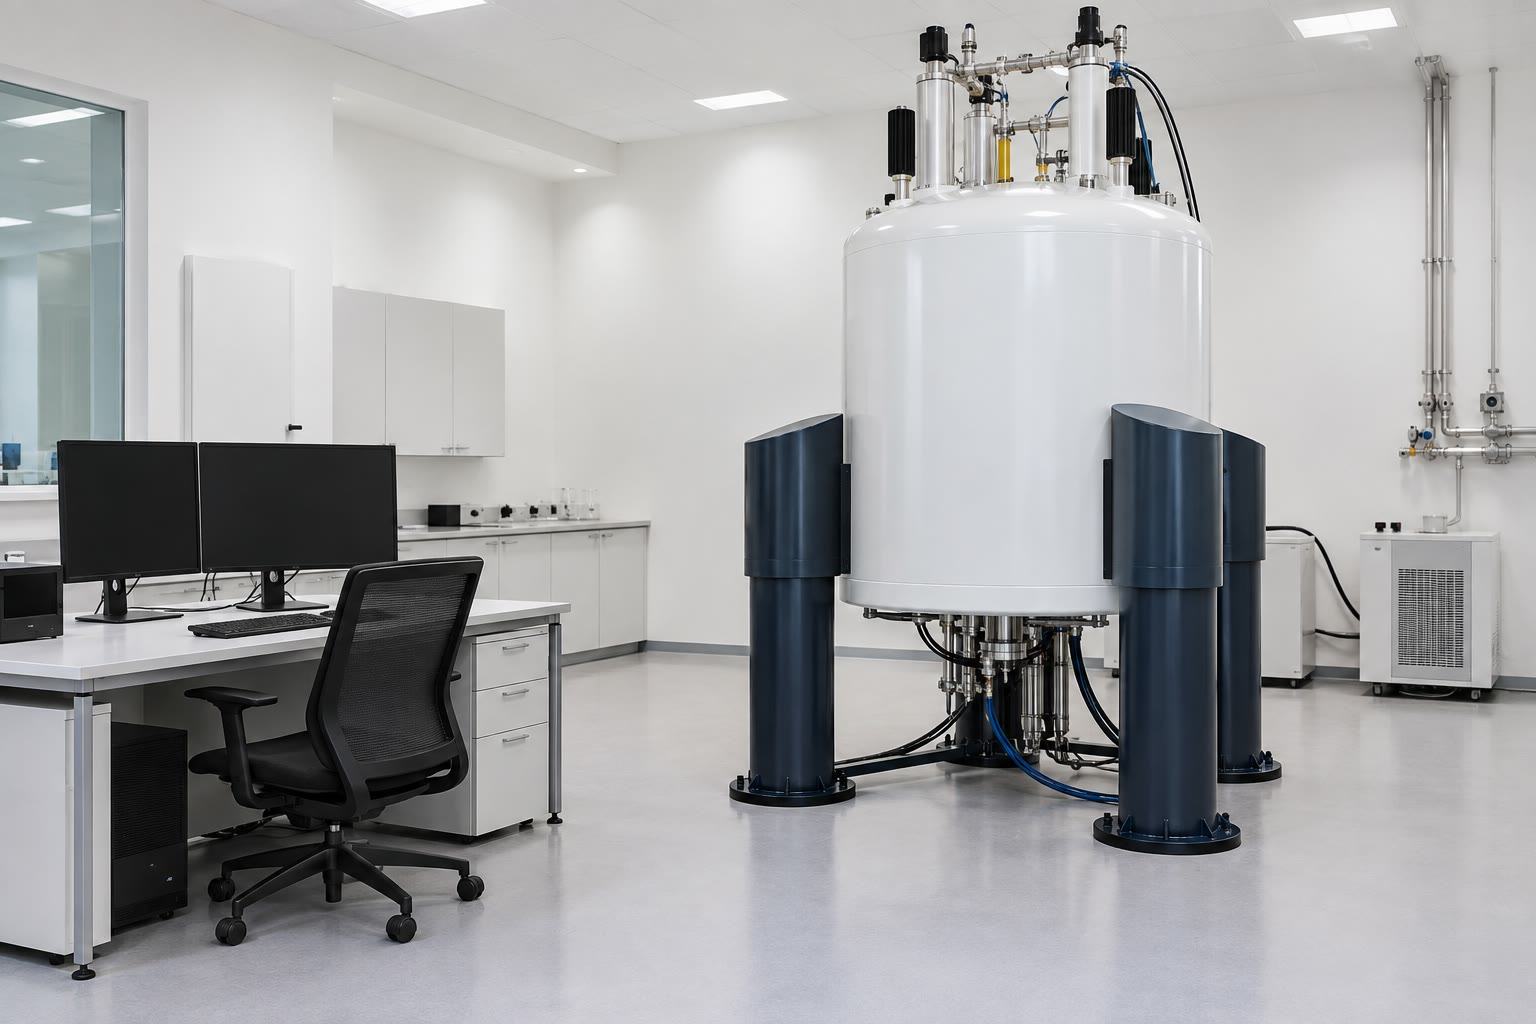
\includegraphics[width=0.5\linewidth]{images/book2/ai/b1-17-nmr.jpg}

{\small مطياف رنين مغناطيسي نووي: تحتوي الأسطوانة الطويلة مغناطيسًا فائق الموصلية
مبرَّدًا بالهيليوم السائل؛ ويُنزَل أنبوب العيّنة إلى
مركزه.}
\end{omfigure}

\section{حل بنية}

\begin{definition}[درجة عدم التشبع]\label{def:b1:structure-spectroscopy:unsaturation}
\emph{درجة عدم التشبع}\index{درجة عدم التشبع} لصيغة
هي عدد الحلقات مضافًا إليه عدد الروابط $\pi$ في
الجزيء.
\end{definition}

\begin{proposition}[درجة عدم التشبع من الصيغة]\label{prop:b1:structure-spectroscopy:unsaturation-formula}
من أجل جزيء $\mathrm{C}_c\mathrm{H}_h\mathrm{N}_n\mathrm{O}_o\mathrm{X}_x$
(X هالوجين)، تكون \omterm{def:b1:structure-spectroscopy:unsaturation}{درجة عدم التشبع}
\[
  D = \frac{2c + 2 + n - h - x}{2} .
\]
\end{proposition}

\begin{proof}
تحمل سلسلة مفتوحة من $c$ كربونًا لا تضم إلا روابط أحادية $2c + 2$
هيدروجينًا. وكل حلقة أو رابطة $\pi$ تنقص اثنين منها. والأكسجين الثنائي التكافؤ
المُدرج في سلسلة لا يغيّر شيئًا؛ والنيتروجين الثلاثي التكافؤ يجلب هيدروجينًا
إضافيًا؛ والهالوجين يحل محل هيدروجين واحد. وعدّ
الهيدروجينات الناقصة والقسمة على اثنين يعطيان $D$.
\end{proof}

\begin{method}[حل بنية]\label{met:b1:structure-spectroscopy:solve-structure}
\begin{enumerate}
  \item احسب $D$ انطلاقًا من الصيغة.
  \item عيّن من طيف الأشعة تحت الحمراء المجموعات الوظيفية (C=O، O--H، N--H،
        C--O) وغياب غيرها.
  \item ومن طيف الرنين المغناطيسي النووي: عدد الإشارات (مجموعات \omterm{def:b1:structure-spectroscopy:chemical-shift}{البروتونات
        المتكافئة})، \omterm{def:b1:structure-spectroscopy:integration}{والتكاملات} (عدد البروتونات في كل مجموعة)، والانزياحات (المجموعات
        المجاورة)، وتعدد الخطوط (عدد الجيران حسب قاعدة $n + 1$)،
        \omterm{def:b1:structure-spectroscopy:coupling}{وثوابت الاقتران} (أي الإشارات متجاورة).
  \item ابنِ أجزاء، وصِل بينها، وتحقق من كل قمة مقابل
        البنية المقترحة؛ واستبعد المتماكبات التي لا توافقها.
\end{enumerate}
\end{method}

\section{تمارين}

\begin{exercise}[$\star$]\label{exo:b1:structure-spectroscopy:1}
محلول صبغة تركيزه \qty{2.0e-5}{mol/L} في خلية طولها \qty{1.00}{cm} له
\omterm{def:b1:structure-spectroscopy:absorbance}{امتصاصية} 0.64 عند قمة امتصاصه. احسب $\varepsilon$،
\omterm{def:b1:structure-spectroscopy:absorbance}{وامتصاصية} محلول أكثر تركيزًا بثلاث مرات.
\end{exercise}

\begin{exercise}[$\star$]\label{exo:b1:structure-spectroscopy:2}
احسب \omterm{def:b1:structure-spectroscopy:unsaturation}{درجة عدم التشبع} لكل من \ce{C6H6} و\ce{C4H8O2} و\ce{C3H7NO}
و\ce{C2H3Cl} و\ce{C10H14O} (الكارفون). واقترح بنية واحدة لكل منها.
\end{exercise}

\begin{exercise}[$\star$]\label{exo:b1:structure-spectroscopy:3}
كم إشارة بروتونية، وبأي \omterm{def:b1:structure-spectroscopy:integration}{تكاملات}، يعطي كل من البروبانون، وحمض
الإيثانويك، و2-ميثيل البروبان و1,2-ثنائي كلورو الإيثان؟
\end{exercise}

\begin{exercise}[$\star$]\label{exo:b1:structure-spectroscopy:4}
تقع إشارة على بعد \qty{1460}{Hz} من رباعي ميثيل السيليكون على
مطياف \qty{400}{MHz}. ما انزياحها؟ وكم تبعد بالهرتز
عند \qty{90}{MHz}؟ ولماذا تفصل المجالات العالية \omterm{def:b1:structure-spectroscopy:coupling}{متعددات الخطوط} فصلًا أفضل؟
\end{exercise}

\begin{exercise}[$\star\star$]\label{exo:b1:structure-spectroscopy:5}
توقّع تعدد خطوط كل إشارة من إشارات 1-برومو البروبان،
\ce{CH3CH2CH2Br}، بافتراض تساوي \omterm{def:b1:structure-spectroscopy:coupling}{ثوابت الاقتران}، والشدّات
النسبية لخطوط الإشارة الوسطى.
\end{exercise}

\begin{exercise}[$\star\star$]\label{exo:b1:structure-spectroscopy:6}
كيف تختلف أطياف الأشعة تحت الحمراء للإيثانول والبروبانون وحمض الإيثانويك
بين 1700 و\qty{3700}{cm^{-1}}؟ وأي مركب وحده يعطي
حزمة C=O وحزمة O--H معًا؟
\end{exercise}

\begin{exercise}[$\star\star$]\label{exo:b1:structure-spectroscopy:7}
متماكبان صيغتهما \ce{C4H8O2}: إيثانوات الإيثيل وبروبانوات الميثيل. توقّع
طيفي الرنين المغناطيسي النووي لهما (الانزياحات تقريبًا، وتعدد الخطوط، \omterm{def:b1:structure-spectroscopy:integration}{والتكاملات})
وبيّن كيف تميّز بينهما.
\end{exercise}

\begin{exercise}[$\star\star$]\label{exo:b1:structure-spectroscopy:8}
مستعينًا بالطيف المحاكى لإيثانوات الإيثيل، اقرأ المسافة بين
خطين من الرباعية بالجزء من المليون وحوّلها إلى هرتز (الطيف
محاكى عند \qty{90}{MHz}). وقارن بالثلاثية.
\end{exercise}

\begin{exercise}[$\star\star$]\label{exo:b1:structure-spectroscopy:9}
مركب \ce{C3H6O} يُظهر حزمة أشعة تحت حمراء قوية عند \qty{1738}{cm^{-1}}
وإشارة رنين وحيدة. عيّنه. وأي متماكب يُظهر حزمة قرب
\qty{2720}{cm^{-1}} وإشارة قرب \qty{9.8}{ppm}؟
\end{exercise}

\begin{exercise}[$\star\star\star$]\label{exo:b1:structure-spectroscopy:10}
برهن قاعدة $n + 1$ في الصيغة الآتية: البروتون المقترن بمجموعتين مختلفتين
من الجيران، $n_1$ بالثابت $J_1$ و$n_2$ بالثابت $J_2$، يعطي $(n_1 +
1)(n_2 + 1)$ خطًا. وحين $J_1 = J_2$، كم خطًا متمايزًا يبقى؟
وطبّق ذلك على \ce{CH2} الوسطى في 1-برومو البروبان.
\end{exercise}

\begin{exercise}[$\star\star\star$]\label{exo:b1:structure-spectroscopy:11}
مركب \ce{C4H10O} لا يعطي أي حزمة أشعة تحت حمراء بين 1700 و1800 لكنه يعطي حزمة عريضة
قرب \qty{3350}{cm^{-1}} في الحالة السائلة، وطيف رنين مغناطيسي نووي فيه ثنائية
(6H)، \omterm{def:b1:structure-spectroscopy:coupling}{ومتعدد خطوط} (1H)، وثنائية (2H) وأحادية عريضة (1H). أوجد
البنية.
\end{exercise}

\begin{exercise}[$\star\star\star$]\label{exo:b1:structure-spectroscopy:12}
بيّن أن \omterm{def:b1:structure-spectroscopy:absorbance}{امتصاصية} خليط من نوعين تحقق $A = \ell(\varepsilon_1c_1
+ \varepsilon_2c_2)$، واشرح كيف تعطي القياسات عند طولين موجيين
التركيزين كليهما.
\end{exercise}

\section{مسألة: جزيء الأناناس}

\begin{problem}[{مسألة نهاية الأسبوع --- تحليل الاحتراق وكثافة
البخار، وطيف الأشعة تحت الحمراء، وطيف الرنين المغناطيسي النووي للبروتون،
وبنية الإستر ذي رائحة الأناناس وكتلته المولية}]
\label{pb:b1:structure-spectroscopy:1}
المجهول سائل لا يحتوي إلا C وH وO. ويعطي احتراق
\qty{0.2500}{g} منه \qty{0.5690}{g} من ثنائي أكسيد الكربون
و\qty{0.2328}{g} من الماء. وكثافة بخاره \qty{3.74}{g/L} عند
\qty{100}{\celsius} و\qty{1.000}{bar}. حزم الأشعة تحت الحمراء في \omterm{def:b1:extent-q-and-k:system}{الطور} الغازي: 2982،
1754، \qty{1182}{cm^{-1}} (قوية)، ولا شيء فوق
\qty{3100}{cm^{-1}}. الرنين المغناطيسي النووي للبروتون (\ce{CDCl3}): 4.13 (رباعية، 2H، $J = \qty{7.2}{Hz}$)،
2.28 (ثلاثية، 2H)، 1.66 (سداسية، 2H)، 1.25 (ثلاثية، 3H، $J = \qty{7.2}{Hz}$)، 0.95
(ثلاثية، 3H) بالجزء من المليون. $M$: C 12.0، H 1.0، O \qty{16.0}{g/mol}؛ $R =
\qty{8.314}{J/(K.mol)}$.
% ledger: ir:ethylbutanoate-CH, ir:ethylbutanoate-CO, ir:ethylbutanoate-COC, nmr:ethylbutanoate-OCH2, nmr:ethylbutanoate-CH2CO, nmr:ethylbutanoate-CH2, nmr:ethylbutanoate-OCH2CH3, nmr:ethylbutanoate-CH3, nmr:ethylbutanoate-J

\begin{center}
\begin{tikzpicture}
\begin{axis}[width=0.86\linewidth, height=4.0cm, xmin=0.6, xmax=4.5, x dir=reverse, ymin=0, ymax=1.15,
  axis x line=bottom, axis y line=none, xlabel={\babelsublr{$\delta$ (ppm)}},
  tick label style={font=\scriptsize}, label style={font=\small}]
\addplot[omDef, thin] table[x=ppm, y=I] {figdata/out/bachelor-1-spectra-nmr-ethylbutanoate.dat};
\end{axis}
\end{tikzpicture}
\end{center}

\medskip
\noindent\textbf{الجزء الأول --- الصيغة.}
\begin{enumerate}
  \item احسب كتلة الكربون في العيّنة.
  \item احسب كتلة الهيدروجين.
  \item استنتج كتلة الأكسجين.
  \item احسب النسب المئوية الكتلية لكل من C وH وO.
  \item أوجد الصيغة التجريبية.
  \item احسب الكتلة المولية انطلاقًا من كثافة البخار (غاز مثالي).
  \item أعطِ الصيغة الجزيئية ودرجة عدم تشبعها.
\end{enumerate}

\medskip
\noindent\textbf{الجزء الثاني --- طيف الأشعة تحت الحمراء.}
\begin{enumerate}[resume]
  \item انسب الحزمة عند \qty{1754}{cm^{-1}}.
  \item ماذا يستبعد غياب الحزم فوق \qty{3100}{cm^{-1}}؟
  \item انسب الحزمة القوية عند \qty{1182}{cm^{-1}}.
  \item انسب الحزمة عند \qty{2982}{cm^{-1}}.
  \item مع \omterm{def:b1:structure-spectroscopy:unsaturation}{درجة عدم التشبع}، أي عائلة من المركبات
        تبقى؟ ولماذا ليس حمضًا كربوكسيليًا، أو كيتونًا مع إيثر، أو
        ثنائي أول حلقيًا؟
\end{enumerate}

\medskip
\noindent\textbf{الجزء الثالث --- طيف الرنين المغناطيسي النووي.}
\begin{enumerate}[resume]
  \item كم مجموعة من \omterm{def:b1:structure-spectroscopy:chemical-shift}{البروتونات المتكافئة}؟ وتحقق من \omterm{def:b1:structure-spectroscopy:integration}{التكامل} الكلي.
  \item فسّر الرباعية عند 4.13 جزءًا من المليون: الجيران والبيئة.
  \item فسّر الثلاثية عند 1.25 جزءًا من المليون. ولماذا تشترك الإشارتان في قيمة
        $J$ نفسها؟
  \item فسّر الثلاثية عند 2.28 جزءًا من المليون.
  \item فسّر السداسية عند 1.66 جزءًا من المليون.
  \item فسّر الثلاثية عند 0.95 جزءًا من المليون.
  \item ابنِ الجزأين اللذين تصفهما هذه الإشارات.
  \item لماذا كانت الإشارتان عند 4.13 و2.28 جزءًا من المليون الأشد إزالةً للحجب؟
\end{enumerate}

\medskip
\noindent\textbf{الجزء الرابع --- البنية.}
\begin{enumerate}[resume]
  \item صِل الجزأين عبر مجموعة الإستر: يوجد احتمالان.
        أيهما يوافق الانزياحات؟
  \item فسّر لماذا لا يناسب بروبانوات البروبيل.
  \item فسّر لماذا لا يناسب إيثانوات البوتيل.
  \item سمِّ المركب وارسم بنيته.
  \item تحقق من كل حزمة أشعة تحت حمراء وكل إشارة رنين مقابل البنية.
  \item اذكر الكتلة المولية لجزيء الأناناس.
\end{enumerate}
\end{problem}
